\documentclass[12pt, a4paper]{article}

\usepackage{amsmath}
\usepackage{amssymb}
\usepackage{amsthm}
\usepackage{graphicx}
\usepackage{booktabs}
\usepackage{geometry}
\usepackage{float}
\usepackage{caption}
\usepackage{array}
\usepackage{xcolor}

\geometry{margin=1in}

\newtheorem{theorem}{Theorem}

\title{\textbf{ME6030 --- Markov Matrix Analysis}\\[0.5em]
\large Manufacturing Plant Workstation Transitions}
\author{Shailesh K \\ me22b192}
\date{April 2026}

\begin{document}

\maketitle

% =========================================================
\section{Problem Setup}
% =========================================================

A manufacturing plant operates three workstations:

\begin{center}
\begin{tabular}{clp{8cm}}
\toprule
\textbf{State} & \textbf{Workstation} & \textbf{Description} \\
\midrule
1 & Machining Centre       & Primary processing of incoming jobs \\
2 & Quality Inspection Bay & Inspection after machining \\
3 & Rework Station         & Correction of defective parts \\
\bottomrule
\end{tabular}
\end{center}

\vspace{0.5em}
The system transitions between states at the end of each production cycle according
to the \textbf{Markov transition matrix} $P$, where $P_{ij}$ denotes the probability
of transitioning \emph{from} State~$j$ \emph{to} State~$i$ in one cycle:

\begin{equation}
  P =
  \begin{bmatrix}
    0.7 & 0.2 & 0.1 \\
    0.3 & 0.5 & 0.2 \\
    0   & 0.3 & 0.7
  \end{bmatrix}
\end{equation}

Every column sums to 1 and all entries are non-negative, so $P$ is a valid
column-stochastic Markov matrix. The governing \textbf{difference equation} is:
\begin{equation}
  \mathbf{z}_{k+1} = P\,\mathbf{z}_k, \qquad \text{with solution} \quad
  \mathbf{z}_k = P^k\,\mathbf{z}_0
\end{equation}
where $\mathbf{z}_0$ is the initial state distribution.

% =========================================================
\section{Proof: $\lambda = 1$ is Always an Eigenvalue of a Markov Matrix}
% =========================================================

\begin{theorem}
Let $P \in \mathbb{R}^{n \times n}$ be column-stochastic, i.e.\
$P_{ij} \geq 0$ and $\sum_{i=1}^{n} P_{ij} = 1$ for all $j$.
Then $\lambda = 1$ is an eigenvalue of $P$.
\end{theorem}

\begin{proof}
Let $\mathbf{1} = [1,\,1,\,\ldots,\,1]^T \in \mathbb{R}^n$.  The column-stochastic
condition says every column of $P$ sums to 1, which is exactly:
\begin{equation}
  \mathbf{1}^T P = \mathbf{1}^T
  \label{eq:lefteig}
\end{equation}
because the $j$-th entry of $\mathbf{1}^T P$ is $\sum_{i=1}^{n} P_{ij} = 1$.
Equation~\eqref{eq:lefteig} says $\mathbf{1}^T$ is a \emph{left} eigenvector of
$P$ with eigenvalue 1.  Transposing both sides:
\begin{equation}
  P^T \mathbf{1} = \mathbf{1}
\end{equation}
so $\mathbf{1}$ is a right eigenvector of $P^T$ with eigenvalue 1.  Since $P$
and $P^T$ share the same characteristic polynomial,
\begin{equation}
  \det(P - \lambda I) = \det\!\left((P-\lambda I)^T\right) = \det(P^T - \lambda I),
\end{equation}
they have identical eigenvalues.  Therefore $\lambda = 1$ is also an eigenvalue
of $P$.  A corresponding right eigenvector $\boldsymbol{\pi}$ satisfying
$P\boldsymbol{\pi} = \boldsymbol{\pi}$ exists; by the Perron--Frobenius theorem it
has strictly positive entries for an irreducible positive stochastic matrix.
\end{proof}

% =========================================================
\section{Eigenvalues of $P$}
% =========================================================

\subsection*{Characteristic Polynomial}

The eigenvalues satisfy $\det(P - \lambda I) = 0$. Expanding the determinant:

\begin{equation}
  \det
  \begin{bmatrix}
    0.7-\lambda & 0.2           & 0.1 \\
    0.3         & 0.5-\lambda   & 0.2 \\
    0           & 0.3           & 0.7-\lambda
  \end{bmatrix} = 0
\end{equation}

Expanding along the first column and simplifying:
\begin{equation}
  -\lambda^3 + 1.9\lambda^2 - 1.07\lambda + 0.17 = 0
  \quad\Longleftrightarrow\quad
  \lambda^3 - 1.9\lambda^2 + 1.07\lambda - 0.17 = 0
\end{equation}

Since $\lambda = 1$ is a guaranteed root (Theorem~1), we factor out $(\lambda - 1)$:
\begin{equation}
  (\lambda - 1)\!\left(\lambda^2 - 0.9\lambda + 0.17\right) = 0
\end{equation}

The quadratic $\lambda^2 - 0.9\lambda + 0.17 = 0$ has discriminant
$\Delta = 0.9^2 - 4(0.17) = 0.81 - 0.68 = 0.13 > 0$, giving two real roots:
\begin{equation}
  \lambda_{2,3} = \frac{0.9 \pm \sqrt{0.13}}{2}
\end{equation}

\subsection*{Numerical Values}

\begin{center}
\begin{tabular}{cccl}
\toprule
& \textbf{Eigenvalue} & $|\lambda_i|$ & \textbf{Note} \\
\midrule
$\lambda_1$ & $1.000000$ & $1.000000$ & Steady-state mode (guaranteed) \\
$\lambda_2$ & $0.630278 = \dfrac{0.9+\sqrt{0.13}}{2}$ & $0.630278$ & Transient mode \\[6pt]
$\lambda_3$ & $0.269722 = \dfrac{0.9-\sqrt{0.13}}{2}$ & $0.269722$ & Transient mode \\
\bottomrule
\end{tabular}
\end{center}

All eigenvalues are real.  Since $|\lambda_2|, |\lambda_3| < 1$, the transient modes
decay geometrically and the system converges to a unique steady state.

% =========================================================
\section{Eigenvectors of $P$}
% =========================================================

\subsection*{Eigenvector for $\lambda_1 = 1$ (Analytical)}

We solve $(P - I)\mathbf{v} = \mathbf{0}$:
\begin{equation}
  P - I =
  \begin{bmatrix}
   -0.3 &  0.2 &  0.1 \\
    0.3 & -0.5 &  0.2 \\
    0   &  0.3 & -0.3
  \end{bmatrix}
\end{equation}

Row 3 gives $0.3\,v_2 - 0.3\,v_3 = 0$, so $v_2 = v_3$.
Row 1 then gives $-0.3\,v_1 + 0.2\,v_2 + 0.1\,v_2 = 0$, i.e.\
$-0.3\,v_1 + 0.3\,v_2 = 0$, so $v_1 = v_2$.
Hence $v_1 = v_2 = v_3$ and the eigenvector is proportional to $\mathbf{1}$:
\begin{equation}
  \mathbf{v}_1 \propto
  \begin{bmatrix} 1 \\ 1 \\ 1 \end{bmatrix}
\end{equation}

\subsection*{Eigenvectors for $\lambda_2$ and $\lambda_3$ (Numerical)}

The remaining eigenvectors are obtained via \texttt{numpy.linalg.eig} (L2-normalised):
\begin{equation}
  \mathbf{v}_2 \approx
  \begin{bmatrix} \phantom{-}0.5988 \\ \phantom{-}0.1813 \\ -0.7801 \end{bmatrix},
  \qquad
  \mathbf{v}_3 \approx
  \begin{bmatrix} \phantom{-}0.2410 \\ -0.7961 \\ \phantom{-}0.5551 \end{bmatrix}
\end{equation}

Both $\mathbf{v}_2$ and $\mathbf{v}_3$ have mixed signs, meaning they represent
oscillatory redistribution between workstations that decays over time.

\begin{figure}[H]
  \centering
  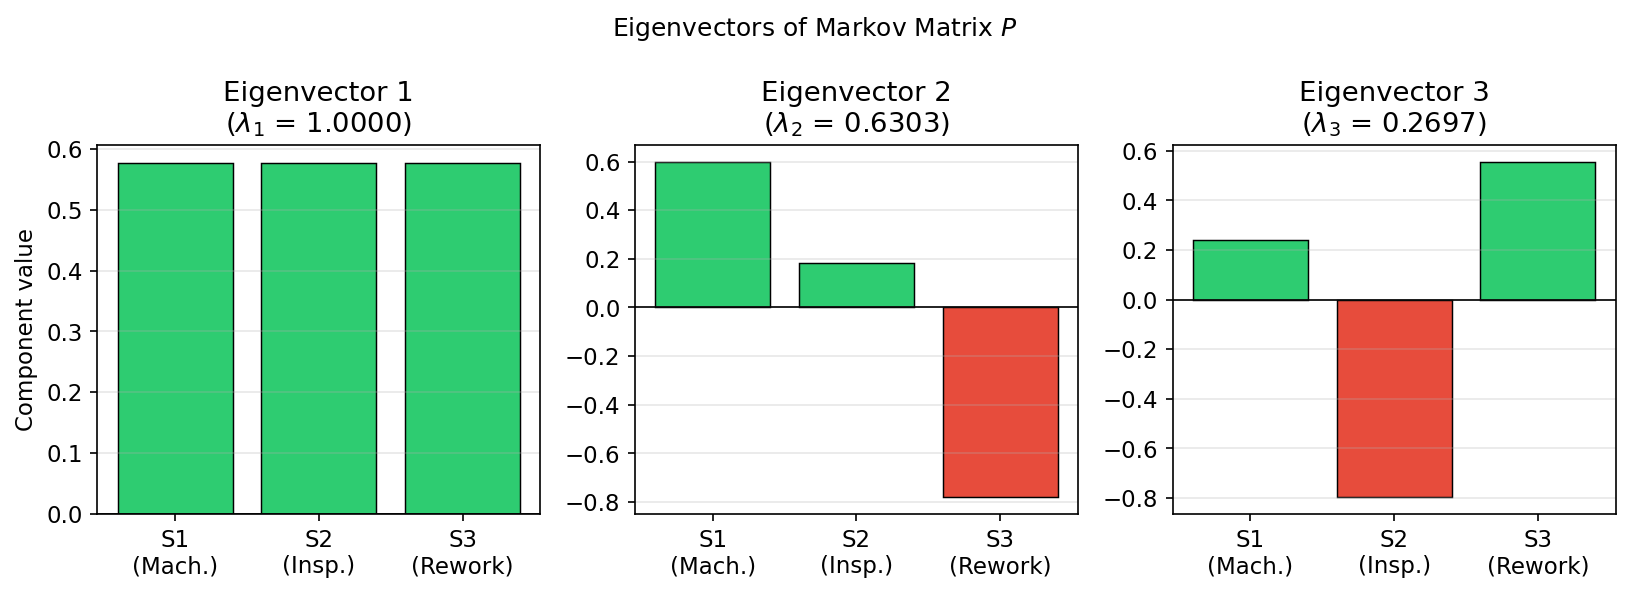
\includegraphics[width=0.95\textwidth]{plots/eigenvectors_bar.png}
  \caption{Components of all three eigenvectors. Eigenvector~1 (all equal positive
    bars) is the uniform steady-state mode. Eigenvectors~2 and~3 have mixed signs
    and represent transient redistribution that decays geometrically.}
  \label{fig:evecs}
\end{figure}

% =========================================================
\section{The $\lambda = 1$ Eigenvector and Its Physical Significance}
\label{sec:ss}
% =========================================================

L1-normalising $\mathbf{v}_1 \propto [1,1,1]^T$ so that its components sum to 1
gives the \textbf{steady-state distribution}:
\begin{equation}
  \boldsymbol{\pi} =
  \frac{1}{3}\begin{bmatrix} 1 \\ 1 \\ 1 \end{bmatrix}
  =
  \begin{bmatrix} 1/3 \\ 1/3 \\ 1/3 \end{bmatrix}
  \approx
  \begin{bmatrix} 0.3333 \\ 0.3333 \\ 0.3333 \end{bmatrix}
\end{equation}

This is an \emph{exact} result confirmed analytically: $v_1 = v_2 = v_3$ forces a
perfectly uniform distribution.  One can verify $P\boldsymbol{\pi} = \boldsymbol{\pi}$
directly since each row of $P$ sums to $0.7+0.2+0.1 = 1$, $0.3+0.5+0.2 = 1$,
$0+0.3+0.7 = 1$, so multiplying $P$ by $[1/3,\,1/3,\,1/3]^T$ returns the same vector.

\textbf{Physical interpretation:} In the long run, the manufacturing system spends
\textbf{exactly equal time at every workstation} --- one-third of all production cycles
at the Machining Centre, one-third at the Inspection Bay, and one-third at the Rework
Station, regardless of initial conditions.  This uniform distribution arises because
the transition probabilities, while asymmetric, are balanced in a way that produces
no preferred long-run state.

\begin{figure}[H]
  \centering
  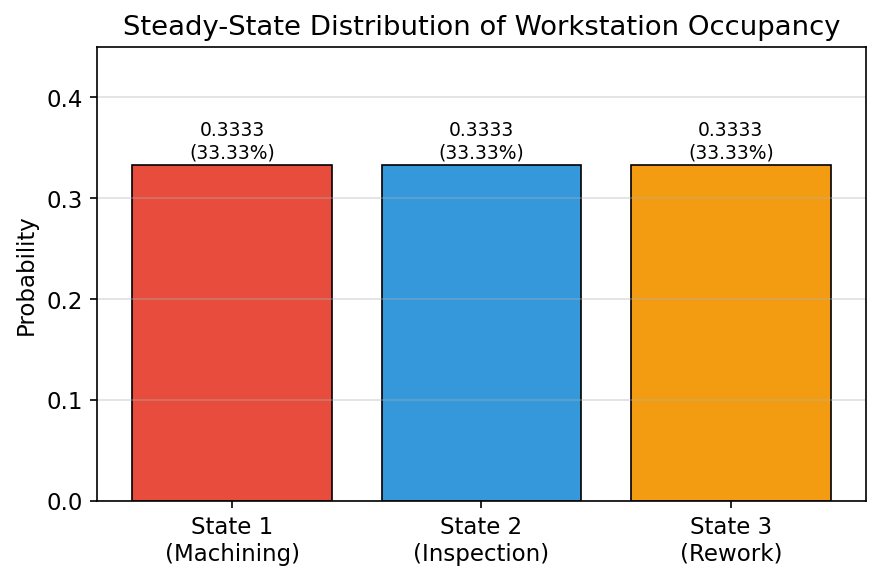
\includegraphics[width=0.62\textwidth]{plots/steady_state_distribution.png}
  \caption{Steady-state workstation occupancy $\boldsymbol{\pi} = [1/3,\,1/3,\,1/3]^T$.
    Each workstation is occupied exactly one-third of the time in the long run.}
  \label{fig:ss}
\end{figure}

% =========================================================
\section{Eigenvalue Magnitudes and Convergence Rate}
% =========================================================

\begin{center}
\begin{tabular}{ccc}
\toprule
$|\lambda_1|$ & $|\lambda_2|$ & $|\lambda_3|$ \\
\midrule
$1.0000$ & $0.6303$ & $0.2697$ \\
\bottomrule
\end{tabular}
\end{center}

Key observations:
\begin{itemize}
  \item $|\lambda_1| = 1$: the steady-state mode persists and defines the long-run
        behaviour.
  \item $|\lambda_2| = 0.6303 < 1$: this transient mode decays as $0.6303^k$.
        After 10 steps it retains only $0.6303^{10} \approx 0.7\%$ of its initial
        amplitude; after 20 steps less than $0.005\%$.
  \item $|\lambda_3| = 0.2697 < 1$: even faster decay; after 5 steps it retains
        only $0.2697^5 \approx 0.14\%$.
  \item The \textbf{spectral gap} $1 - |\lambda_2| = 0.3697$ governs the worst-case
        rate of convergence.  A larger gap means faster convergence.
\end{itemize}

\begin{figure}[H]
  \centering
  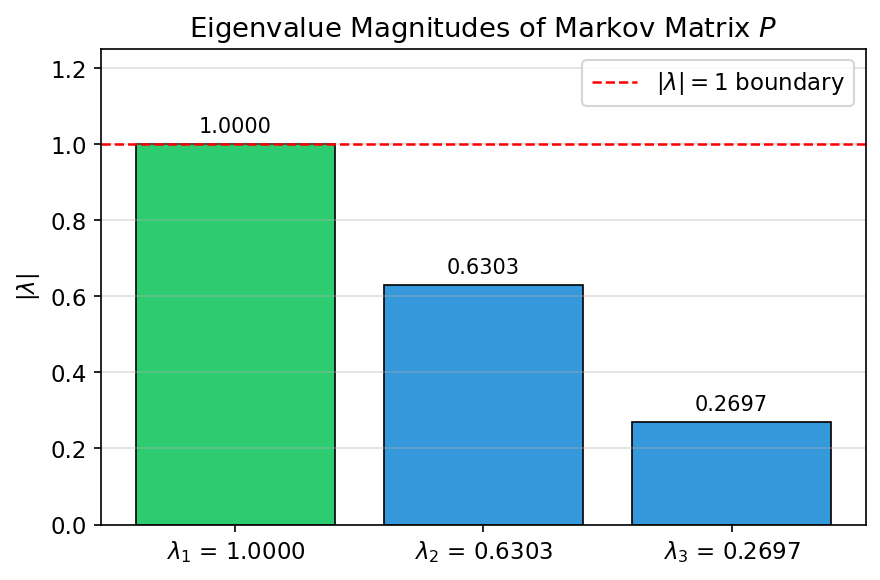
\includegraphics[width=0.62\textwidth]{plots/eigenvalue_magnitudes.png}
  \caption{Magnitudes of the three eigenvalues. $\lambda_1 = 1$ (green) lies on the
    unit-circle boundary; $\lambda_2$ and $\lambda_3$ (blue) are strictly inside,
    ensuring asymptotic convergence to the steady state.}
  \label{fig:emags}
\end{figure}

% =========================================================
\section{Steady-State Analysis: $\mathbf{z}_k$ for Large $k$}
% =========================================================

\subsection*{Analytical Result}

Any initial distribution $\mathbf{z}_0$ decomposes into the eigenbasis:
\begin{equation}
  \mathbf{z}_0 = c_1\,\mathbf{v}_1 + c_2\,\mathbf{v}_2 + c_3\,\mathbf{v}_3
\end{equation}

Applying $P$ repeatedly and using $P\mathbf{v}_i = \lambda_i\mathbf{v}_i$:
\begin{equation}
  \mathbf{z}_k = P^k\mathbf{z}_0
    = c_1\,\underbrace{\lambda_1^k}_{=\,1}\mathbf{v}_1
    + c_2\,\underbrace{(0.6303)^k}_{\to\,0}\mathbf{v}_2
    + c_3\,\underbrace{(0.2697)^k}_{\to\,0}\mathbf{v}_3
\end{equation}

As $k \to \infty$ both transient terms vanish:
\begin{equation}
  \lim_{k\to\infty}\mathbf{z}_k = c_1\,\mathbf{v}_1 = \boldsymbol{\pi}
  = \begin{bmatrix} 1/3 \\ 1/3 \\ 1/3 \end{bmatrix}
\end{equation}

The matrix power converges to the rank-1 matrix
$P^\infty = \boldsymbol{\pi}\,\mathbf{1}^T$, i.e.\ every column of $P^k$ tends
to $\boldsymbol{\pi}$.  The long-run state is therefore
\textbf{independent of the initial condition} $\mathbf{z}_0$.

\subsection*{Numerical Verification ($k = 10\,000$)}

Starting from $\mathbf{z}_0 = [1,\,0,\,0]^T$ (all jobs initially at the machining
centre) and iterating $\mathbf{z}_{k+1} = P\,\mathbf{z}_k$ for $10\,000$ steps:

\begin{equation}
  \mathbf{z}_{10000} =
  \begin{bmatrix} 0.33333333 \\ 0.33333333 \\ 0.33333333 \end{bmatrix},
  \qquad
  \left|\mathbf{z}_{10000} - \boldsymbol{\pi}\right| < 10^{-15}
\end{equation}

The simulation confirms convergence to machine-precision accuracy, consistent with
the analytical prediction.

\begin{figure}[H]
  \centering
  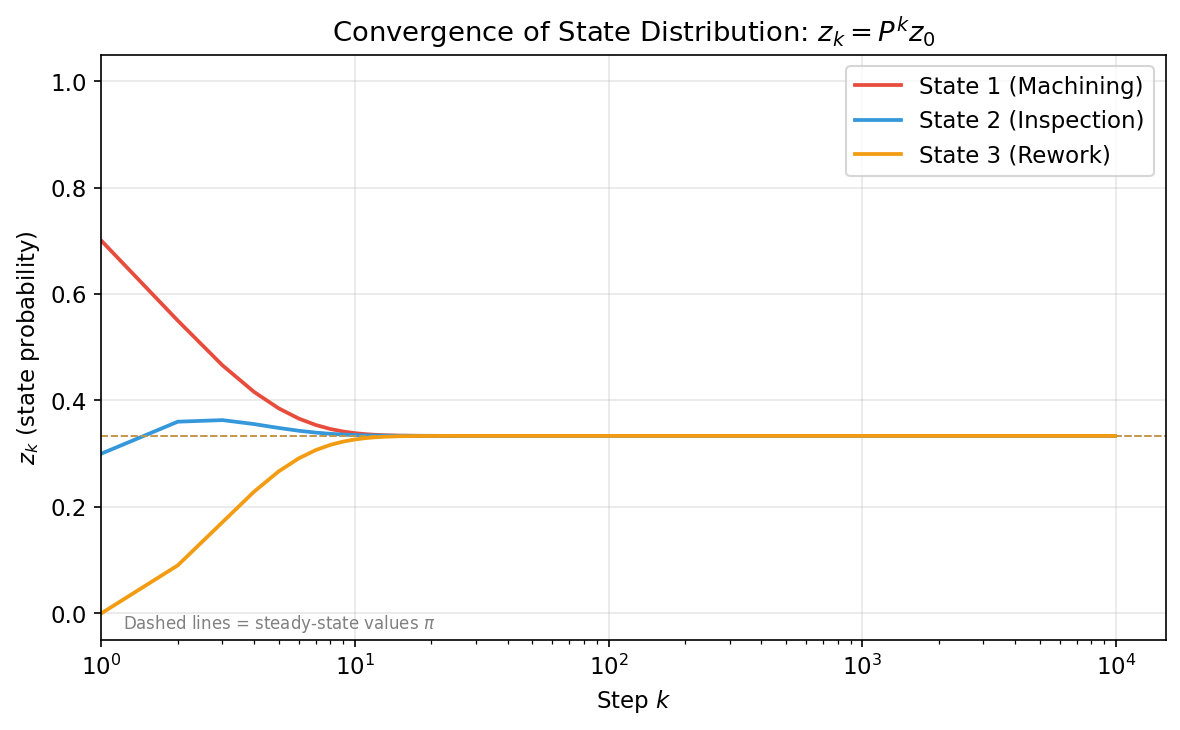
\includegraphics[width=0.85\textwidth]{plots/convergence_all_states.png}
  \caption{Evolution of $\mathbf{z}_k$ over $10\,000$ steps (log scale on $k$).
    All three state probabilities converge to $1/3$ (dashed lines).  Convergence is
    essentially complete by $k \approx 15$--$20$ steps, consistent with the spectral
    gap of $1 - |\lambda_2| = 0.3697$.}
  \label{fig:conv}
\end{figure}

\subsection*{Physical Interpretation}

The system forgets its initial conditions rapidly --- within roughly 15--20 production
cycles, the workstation distribution is indistinguishable from the uniform steady state
$\boldsymbol{\pi}$.  Practically, this means long-run capacity planning is
straightforward: each of the three workstations must be resourced to handle
\textbf{one-third of the total throughput}, irrespective of how jobs enter the plant.

\end{document}
